\chapter{Transforms related to the discrete Fourier transform}
\label{chap-extension-trans-fourier}
\chapteroverview{The Fourier transform belongs to a wider family of useful
transforms. The Hartley transform provides a real kernel, the Z transform
encodes recurrences and filter stability, and the chirp algorithm evaluates
spectra on flexible frequency grids. We develop their algebraic identities
and fast algorithms, while distinguishing exact finite sums from numerical
approximations to continuous signals.}

\section{Hartley transform}
\label{sect1-trans-hartley}
\index{Hartley transform}\index{Hartley@\nompropreindex{Hartley}}
The Hartley transform represents a real signal by real coefficients without
losing phase information. Like the DFT, it has a fast algorithm and can be
used to compute convolutions. It is an alternative representation of the
same information, rather than a uniformly faster replacement for a real-input
FFT. Bracewell~\cite{bracewell} develops this viewpoint in detail.

\subsection{Definition and first properties}
\begin{defn}[Discrete Hartley transform]
\label{notation-58}\label{notation-59}
For $f\in\CC^N$, define
\begin{equation}
\label{eq-defn-transfo-hartley}
 \Hh(f)[k]=\sum_{n=0}^{N-1}f[n]\cas\left(\frac{2\pi nk}{N}\right),
 \qquad 0\leq k<N,
\end{equation}
where $\cas(x)=\cos x+\sin x=\sqrt2\cos(x-\pi/4)$.
The map is complex-linear, and maps $\RR^N$ into $\RR^N$.
\end{defn}
Its continuous counterpart, with frequency measured in cycles per unit,
is $\Hh f(s)=\int_\RR f(x)\cas(2\pi sx)\d x$ for $f\in L^1(\RR)$.

\begin{prop}[Inversion]
\label{prop-ptes-transfo-hartley}
\index{Inversion formula}
The Hartley transform satisfies $\Hh^2=N\Id$. Thus
$\Hh^{-1}=\Hh/N$, and $\Hh/\sqrt N$ is orthogonal on $\RR^N$
and unitary on $\CC^N$.
\end{prop}
\begin{proof}
The identity
\begin{equation}
\label{eqn-proof-inversion-hartley}
 \cas\alpha\cas\beta=\cos(\alpha-\beta)+\sin(\alpha+\beta)
\end{equation}
and the sums of roots of unity give, for $0\leq n,n'<N$,
\begin{equation}
\label{eq-orthogonalite-cas}
 \sum_{k=0}^{N-1}\cas\left(\frac{2\pi nk}{N}\right)
 \cas\left(\frac{2\pi n'k}{N}\right)=N\delta_n^{n'}.
\end{equation}
The sine sum is zero, and the cosine sum is $N$ if $n=n'$ and zero
otherwise. The matrix of $\Hh$ is real and symmetric, so this identity
proves both assertions.
\end{proof}

\begin{prop}[Relation to the DFT]
For real $f$, with the negative exponential in the DFT,
\begin{equation}
\label{eq-relation-tfd-hartley}
 \Hh(f)=\realp\Ff(f)-\imagp\Ff(f),\qquad
 \Ff(f)=\psym{\Hh(f)}-\imath\pasym{\Hh(f)}.
\end{equation}
Here $g^\sharp[k]=g[-k]$, with indices modulo $N$,
$\psym g=(g+g^\sharp)/2$, and $\pasym g=(g-g^\sharp)/2$.
\end{prop}
\begin{proof}
Take real and imaginary parts in the DFT formula. The cosine contribution
is symmetric in $k$, and the sine contribution is antisymmetric.
\end{proof}
For complex $f$, the first formula must instead be written in a
complex-linear form:
\[
 \Hh(f)=\tfrac12\bigl((1+\imath)\Ff(f)
                    +(1-\imath)\Ff(f)^\sharp\bigr).
\]
For real input, the Fourier symmetry $\wh f[-k]=\overline{\wh f[k]}$
explains why $N$ real Hartley coefficients suffice. Real-input FFT routines
also exploit this symmetry. Their relative speed and memory use depend on
the implementation; the Hartley formulation alone gives no universal
factor-of-two advantage or improvement in rounding error.

\subsection{Fast Hartley transform}
\label{sect2-algo-de-calcul-hartley}
\index{Algorithm!FHT}\index{FHT}
Let $N=2M$, $f^0[n]=f[2n]$, and $f^1[n]=f[2n+1]$. Splitting the sum gives
\begin{equation}
\label{eq-decomposition-transfo-hartley1}
 \Hh_N(f)[k]=\sum_{n=0}^{M-1}f^0[n]\cas\frac{2\pi nk}{M}
 +\sum_{n=0}^{M-1}f^1[n]\cas\left(\frac{2\pi nk}{M}+\frac{2\pi k}{N}\right).
\end{equation}
The addition formula
\begin{equation}
\label{eq-prop-function-case}
 \cas(\alpha+\beta)=\cas\alpha\cos\beta+\cas(-\alpha)\sin\beta
\end{equation}
expresses the odd-index sum using the length-$M$ Hartley transform and
its reversal. More generally, set
\begin{equation}
\label{eq-decomposition-transfo-hartley2}
 (\chi_M^x a)[j]=a[j]\cos\frac{2\pi jx}{M}
                 +a[-j]\sin\frac{2\pi jx}{M}.
\end{equation}
Writing $E=\Hh_M(f^0)$ and $O=\Hh_M(f^1)$, we obtain
\begin{align}
 \Hh_N(f)[k]&=E[k]+(\chi_M^{1/2}O)[k],\label{eq-decomposition-transfo-hartley}\\
 \Hh_N(f)[k+M]&=E[k]-(\chi_M^{1/2}O)[k],\label{eq-decomposition-transfo-hartley-2}
\end{align}
for $0\leq k<M$. Recursion, starting from $N=1$, gives an $O(N\log N)$
algorithm when $N$ is a power of two. The implementation in
Section~\ref{sect1-listing-fht} uses real arithmetic for real inputs.
Ullmann~\cite{ullmann} describes iterative arrangements that group the
coupled frequencies into larger butterflies.

\paragraph{Zero padding.}
Appending zeros evaluates the finite-record Hartley spectrum at more
frequencies. It does not add measurements or change the information in the
signal. Approximating a continuous transform additionally requires a
sampling model and a quadrature normalization. Figure~\ref{fig-comparison-fht-fft}
compares the Hartley spectrum of a triangular signal with the real part of
its Fourier spectrum; their difference is the negative imaginary part.
\begin{figure}[tbp]
\centering
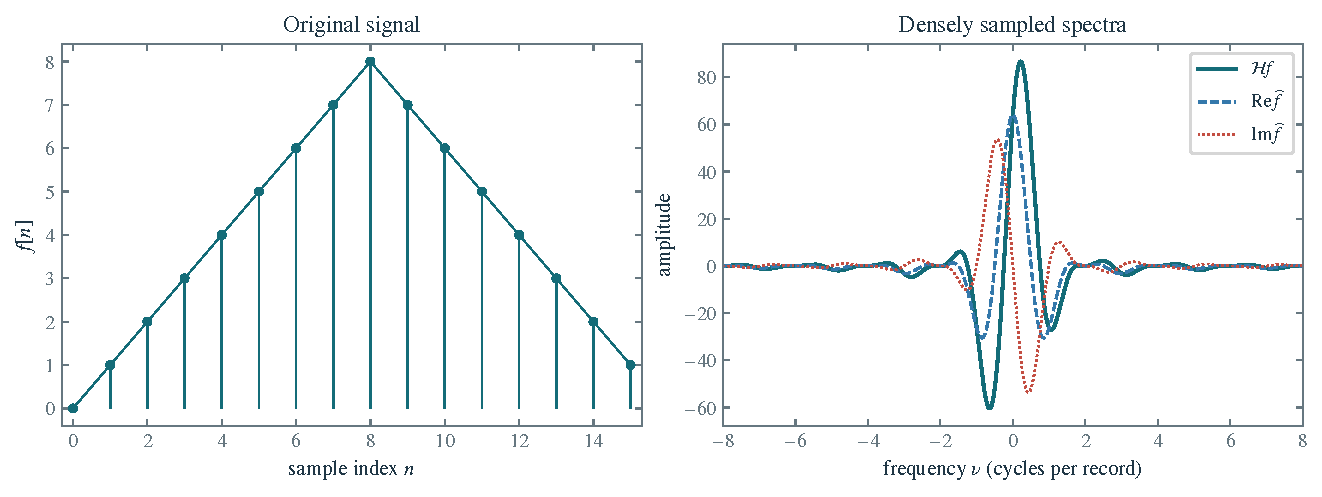
\includegraphics[width=\linewidth]{figures/chapter-related-transforms/hartley-and-fourier/figure.pdf}
\caption{A triangular signal and its densely evaluated Fourier and Hartley spectra. The Hartley spectrum equals the real part minus the imaginary part of the DFT. Zero padding changes only the frequency grid.}
\label{fig-comparison-fht-fft}
\end{figure}

\subsection{Convolution by Hartley transforms}
\label{sect2-usage-hartley-convolution}
\begin{prop}[Hartley convolution formula]
\index{Convolution!by Hartley transform}
For the unnormalized circular convolution of $a,b\in\RR^N$, let
$c=\Hh(a)$ and $d=\Hh(b)$. Then
\[
 \Hh(a*b)[k]=\tfrac12\bigl(c[k](d[k]+d[-k])
                         +c[-k](d[k]-d[-k])\bigr).
\]
\end{prop}
\begin{proof}
Reindex the finite sums and use the addition formula:
\begin{align*}
 \Hh(a*b)[k]
 &=\sum_{l,m}a[l]b[m]\cas\frac{2\pi k(l+m)}{N}\\
 &=d[k]\sum_l a[l]\cos\frac{2\pi kl}{N}
   +d[-k]\sum_l a[l]\sin\frac{2\pi kl}{N}.
\end{align*}
Substitute $\cos x=(\cas x+\cas(-x))/2$ and
$\sin x=(\cas x-\cas(-x))/2$, then rearrange.
\end{proof}
The function \texttt{hartley\_convolution}, in
Section~\ref{sect1-listing-fht}, applies this formula and divides the
final Hartley transform by $N$.

\paragraph{Self-convolution and autocorrelation.}
These are different operations. For $c=\Hh(a)$,
\[
 \Hh(a*a)[k]=c[k]c[-k]+\tfrac12(c[k]^2-c[-k]^2),
\]
whereas the real circular autocorrelation $a*a^\sharp$ satisfies
\[
 \Hh(a*a^\sharp)[k]=|\Ff(a)[k]|^2
                 =\tfrac12(c[k]^2+c[-k]^2).
\]

\section{Z transform and applications}
\label{sect1-trans-Z}
The Z transform encodes a sequence as a Laurent series. Delays become
powers of $z^{-1}$, convolutions become products, and linear recurrences
become rational functions. The region of convergence remains part of the
transform, even when the resulting function is rational.
See~\cite{wich,demengel,cartan-holo} for analytic background and
\cite{knuth-concrete,generatingfunctionology} for generating-function methods.

\subsection{Definition and basic properties}
\label{sect2-defn-trans-Z}
\begin{defn}[Bilateral Z transform]
\label{notation-60}\index{Z transform}\index{Laurent series}
For a sequence $f\in\CC^\ZZ$, define
\begin{equation}
\label{eq-trans-Z-defn}
 \Zz(f)(z)=\sum_{n\in\ZZ}f[n]z^{-n}
\end{equation}
at the points $z\ne0$ where the series converges absolutely.
\end{defn}
If the convergence set has nonempty interior, that interior is an annulus
$r<|z|<R$, with $0\leq r<R\leq\infty$. The series converges locally
uniformly there and defines a holomorphic function. Convergence on its
boundary circles must be checked separately. The interior may be empty:
for example, $f[n]=(1+|n|)^{-2}$ gives absolute convergence only on $|z|=1$.
A finite sequence has a Laurent-polynomial transform and no convergence
issue for $z\ne0$.

\begin{exmp}
The causal constant sequence $u[n]=1$ for $n\geq0$ and zero otherwise has
\[
 \Zz(u)(z)=\frac1{1-z^{-1}},\qquad |z|>1.
\]
If $b\ne0$ and $|a|<|b|$, the sequence equal to $a^n$ for $n\geq0$
and $b^n$ for $n<0$ has transform
\[
 \frac1{1-a/z}+\frac1{1-z/b}-1,
 \qquad |a|<|z|<|b|.
\]
Both formulas follow by summing geometric series in their stated regions.
\end{exmp}

\begin{prop}[Z-transform rules]
\label{prop-prte-z-trans}
Besides linearity, the following identities hold wherever the relevant
series converge absolutely; the derivative formula holds in the open
annulus of convergence:
\begin{align*}
 \Zz(f\star g)&=\Zz(f)\Zz(g),&
 (f\star g)[n]&=\sum_m f[m]g[n-m],\\
 \Zz\bigl(f[\,\cdot-k]\bigr)(z)&=z^{-k}\Zz(f)(z),&
 \Zz\bigl(nf[n]\bigr)(z)&=-z\frac{d}{dz}\Zz(f)(z).
\end{align*}
\end{prop}
\begin{proof}
At a common point of absolute convergence,
\[
 \sum_{m,l}|f[m]g[l]z^{-(m+l)}|
 =\left(\sum_m|f[m]z^{-m}|\right)
  \left(\sum_l|g[l]z^{-l}|\right)<\infty.
\]
Fubini's theorem therefore permits grouping the terms by $n=m+l$,
which proves the convolution rule. Reindexing proves the delay rule;
termwise differentiation of the Laurent series proves the last identity.
\end{proof}
The sequence can be recovered by coefficient extraction. For any circle
$|z|=\rho$ contained in the annulus, oriented counterclockwise,
\[
 f[n]=\frac1{2\pi\imath}\int_{|z|=\rho}\Zz(f)(z)z^{n-1}\d z.
\]

\subsection{Recursive filters}
\label{sect2-application-trans-z-filters}
\begin{defn}[Causal recursive filter]
\label{notation-61}\index{Filter!recursive}
Given coefficients $a_0,\ldots,a_k$ and $b_1,\ldots,b_l$, define
$y=\Phi_a^b(x)$ recursively by
\begin{equation}
\label{eq-defn-recursive-filter}
 y[n]=\sum_{j=0}^k a_jx[n-j]+\sum_{j=1}^l b_jy[n-j],\qquad n\geq0,
\end{equation}
with $x[n]=y[n]=0$ for $n<0$. This is the zero-state convention.
\end{defn}
The rule is linear and causal. Its impulse response $h=\Phi_a^b(\delta_0)$
satisfies $y=h\star x$. At fixed filter order, computing the first $N$
outputs costs $O(N)$ operations. The impulse response is often infinite,
hence the term \emph{IIR filter}; special coefficient choices or
cancellations can also produce a finite impulse response.
Applying the delay rule gives the transfer function
\[
 H(z)=\Zz(h)(z)=\frac{A(z^{-1})}{B(z^{-1})},\qquad
 A(q)=\sum_{j=0}^k a_jq^j,\quad B(q)=1-\sum_{j=1}^l b_jq^j.
\]
For a causal impulse response, its Laurent expansion is taken about
infinity. Nonzero initial conditions add a separate response; they cannot
be dropped when transforming a recurrence.

\begin{exmp}[A first-order filter]
\begin{equation}
\label{eq-recurrence-1st-order}
 y[n]=x[n]+\alpha y[n-1]
\end{equation}
has the causal impulse response $h[n]=\alpha^n$ for $n\geq0$ and zero
otherwise. Its transform is $H(z)=1/(1-\alpha z^{-1})$, with $|z|>|\alpha|$,
and it is stable precisely when $|\alpha|<1$. For $\alpha\ne0$, the same
rational expression also represents the \emph{anticausal} sequence
$h[n]=-\alpha^n$ for $n<0$ and zero otherwise, now in $|z|<|\alpha|$.
That sequence is absolutely summable precisely when $|\alpha|>1$.
The rational expression without its region of convergence does not
identify the impulse response.
\end{exmp}

\begin{prop}[Poles and stability]
\label{prop-poles-stability}\index{Pole}\index{Stability}
A causal rational zero-state filter is bounded-input, bounded-output
stable if and only if every pole of its \emph{reduced} transfer function
has modulus strictly less than one.
\end{prop}
\begin{proof}
By the convolution stability criterion in
Section~\ref{sect2-responses-stability}, stability is equivalent to
$\sum_{n\geq0}|h[n]|<\infty$. In that case the series for $H$ is uniformly
convergent and bounded on $|z|\geq1$. It is holomorphic for $|z|>1$ and
continuous on the unit circle. A pole of the reduced rational function
cannot lie in this region, including its boundary.
Conversely, partial fractions at poles of modulus less than one express
$h[n]$ as a finite sum of polynomially weighted decaying geometric
sequences, together with a finitely supported sequence. Each is absolutely
summable, which proves stability.
\end{proof}
This criterion concerns the zero-state input-output map. Cancelling an
unstable pole algebraically can hide an unstable internal mode in a
particular recurrence with nonzero initial state.

\subsection{Design by poles and zeros}
A notch filter suppresses selected frequencies by placing zeros on the
unit circle. For $\theta=\pi/4$ and $r=0.9$, consider
\[
 H(z)=\frac{(z-e^{\imath\theta})(z-e^{-\imath\theta})}
              {(z-re^{\imath\theta})(z-re^{-\imath\theta})}
      =\frac{z^2-\sqrt2z+1}{z^2-0.9\sqrt2z+0.81}.
\]
Its poles lie strictly inside the unit circle. In the notation of
\eqref{eq-defn-recursive-filter}, its coefficients are
\[
 (a_0,a_1,a_2)=(1,-\sqrt2,1),\qquad
 (b_1,b_2)=(0.9\sqrt2,-0.81).
\]
\begin{figure}[tbp]
\centering
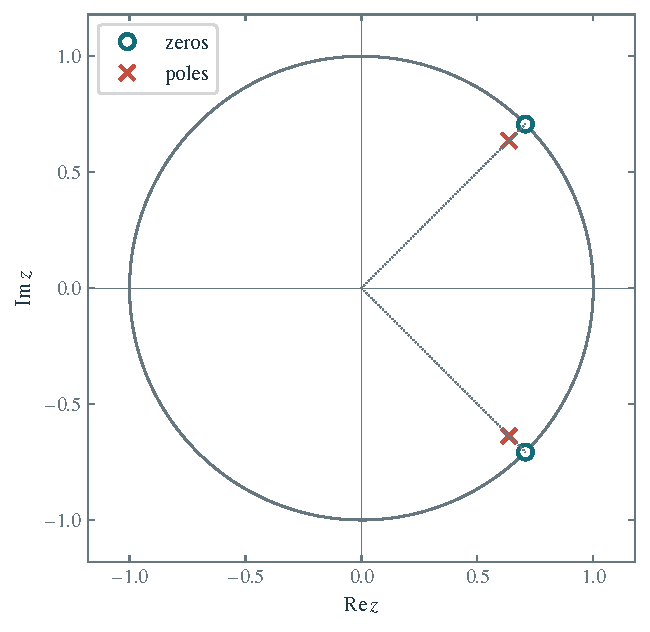
\includegraphics[width=.58\linewidth]{figures/chapter-related-transforms/notch-poles-and-zeros/figure.pdf}
\caption{Zeros on the unit circle and poles at radius $0.9$ for a notch filter at angular frequencies $\pm\pi/4$. Circles mark zeros; crosses mark poles.}
\label{fig-location-poles-notch-filter}
\end{figure}
The frequency response is $\omega\mapsto H(e^{\imath\omega})$.
Its modulus is the gain, while its argument records the phase shift.
One can compute the impulse response directly from the recurrence and
then approximate the response by truncating its Fourier series. Conversely,
an inverse DFT of $N$ equally spaced response values produces the
periodized impulse response $\sum_l h[n+lN]$, not an exact truncation.
For a stable filter, the discrepancy decreases as the decaying tail becomes
negligible.
\begin{figure}[tbp]
\centering
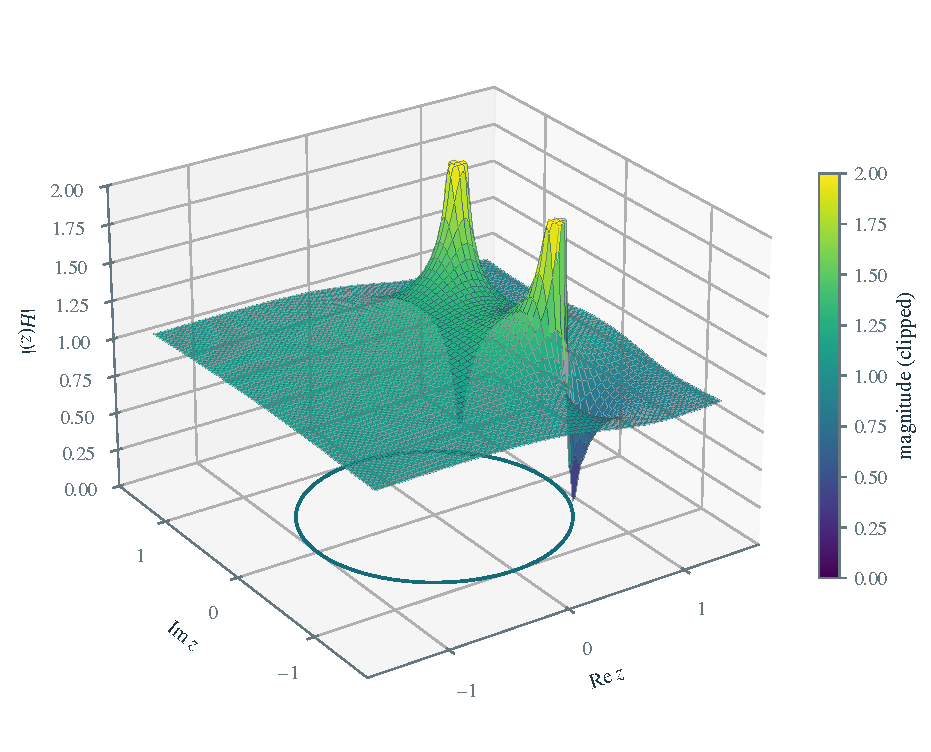
\includegraphics[width=.8\linewidth]{figures/chapter-related-transforms/notch-transfer-surface/figure.pdf}
\caption{Magnitude of the rational notch-filter transfer function in the complex plane. Values above two are clipped to reveal the zeros and pole neighborhoods. The causal Laurent series converges for $|z|>0.9$.}
\label{fig-notch-filter-trans-z}
\end{figure}
\begin{figure}[tbp]
\centering
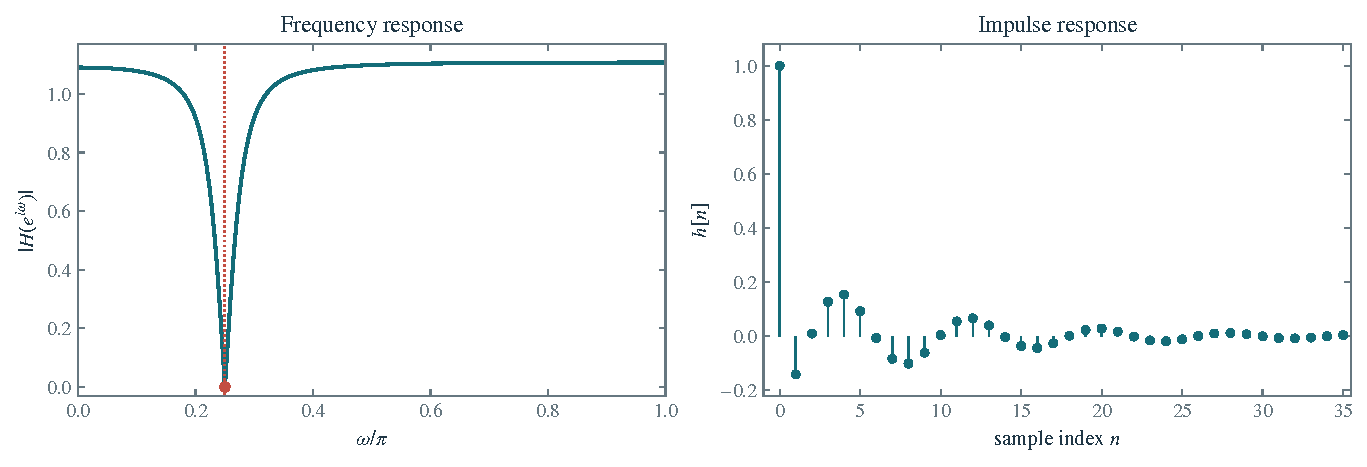
\includegraphics[width=\linewidth]{figures/chapter-related-transforms/notch-responses/figure.pdf}
\caption{Frequency-response magnitude and causal impulse response of the notch filter. The response vanishes at angular frequency $\pi/4$.}
\label{fig-notch-filter-rep-imp-freq}
\end{figure}

A real rational transfer function factors into real first- and second-order
sections, which can be applied in cascade. A partial-fraction decomposition
instead gives parallel branches, together with any polynomial part.
Repeated poles require terms with powers of their irreducible factors;
these terms cannot all be treated as simple first- or second-order
fractions. Exercise~\ref{exo-calcul-spline-iir} illustrates both
arrangements for a spline prefilter.

\subsection{Connection with analog filtering}
\index{Filter!analog}\index{RLC circuit}
Analog filters act on continuous-time signals and are described by
differential equations. Digital filters use difference equations. To connect
the two, consider a series RLC circuit with input voltage $V_e$ and output
$V_s$ across the resistor. Writing $V_s=RI$ and differentiating Kirchhoff's
voltage law gives
\begin{equation}
\label{eq-equation-circuit-rlc}
 V_e'(t)=\frac1{RC}V_s(t)+V_s'(t)+\frac LR V_s''(t).
\end{equation}
\begin{figure}[tbp]
\centering
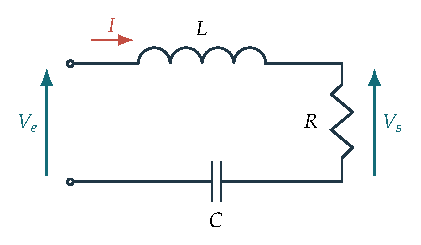
\includegraphics[width=.68\linewidth]{figures/chapter-related-transforms/rlc-circuit/figure.pdf}
\caption{A series RLC circuit, with the output voltage $V_s$ measured across the resistor and the input $V_e$ across the two left terminals.}
\label{fig-circuit-rlc}
\end{figure}

\begin{defn}[Laplace transform]
\label{notation-62}\index{Laplace transform}
For a causal function $f$, its Laplace transform is
$\Ll(f)(s)=\int_0^\infty f(t)e^{-st}\d t$ wherever the integral
converges absolutely.
\end{defn}
With zero initial conditions, differentiation corresponds to multiplication
by $s$. For nonzero initial conditions it also contributes boundary terms;
for instance $\Ll(f')(s)=s\Ll(f)(s)-f(0^+)$. The zero-state transfer function
of the circuit is therefore
\[
 K(s)=\frac{s}{1/(RC)+s+(L/R)s^2}.
\]
Approximate each derivative by a backward difference with time step
$\Delta>0$. If $q=z^{-1}$ denotes a one-step delay, this substitutes
$s=(1-q)/\Delta$ into $K$ and gives
\[
 H(z)=\frac{1-q}
 {\Delta/(RC)+1+L/(R\Delta)-(1+2L/(R\Delta))q+Lq^2/(R\Delta)}.
\]
Equivalently, the sampled voltages satisfy the finite-difference equation
\begin{align*}
 \frac{V_e[n]-V_e[n-1]}\Delta
 &=\frac{V_s[n]}{RC}+\frac{V_s[n]-V_s[n-1]}\Delta\\
 &\quad+\frac{L}{R\Delta^2}
       \bigl(V_s[n]-2V_s[n-1]+V_s[n-2]\bigr).
\end{align*}
The discretization approximates the analog dynamics. Its resulting
recurrence and rational transfer function are exact descriptions of the
digital filter. Other discretizations give different digital filters;
Exercise~\ref{exo-meth-quadratures-recursive-filter} examines this choice
for an integrator.

\section{Vector Z transform and the chirp algorithm}
\label{sect1-trans-Z-vector}
\subsection{A fast evaluation algorithm}
\label{sect2-algo-trans-z}
\begin{defn}[Vector Z transform]
\label{notation-63}\index{Z transform!vector}
For $z\in\CC\setminus\{0\}$ and $f\in\CC^N$, define
\begin{equation}
\label{eq-defn-z-transform-vector}
 \Gg_z(f)[n]=\sum_{k=0}^{N-1}f[k]z^{-nk},\qquad 0\leq n<N.
\end{equation}
\end{defn}
These are exact evaluations of the finite Z transform at
$1,z,z^2,\ldots,z^{N-1}$. The associated Vandermonde matrix is invertible
exactly when these points are distinct, or equivalently
$z^d\ne1$ for $1\leq d<N$. If $|z|=1$, the evaluation points lie on a circle;
otherwise they follow a logarithmic spiral.

Choose one logarithm $L$ of $z$ and use it consistently. The identity
$nk=(n^2+k^2-(n-k)^2)/2$ yields
\[
 \Gg_z(f)[n]=e^{-Ln^2/2}\sum_{k=0}^{N-1}h[k]g[n-k],\qquad
 h[k]=f[k]e^{-Lk^2/2},\quad g[j]=e^{Lj^2/2}.
\]
Thus a diagonal scaling, a Toeplitz product, and a second diagonal scaling
replace the dense Vandermonde product. The sign of the chirp kernel is
positive. Although the factors involve half-integer exponents, the final
integer powers $z^{-nk}$ are independent of the chosen logarithm.

To compute $M$ outputs, choose an FFT length $Q\geq N+M-1$. Place
$g[j]$ at index $j\bmod Q$ for $-(N-1)\leq j\leq M-1$, and pad $h$
with zeros to length $Q$. The first $M$ entries of their circular convolution
are the desired sums: every difference $n-k$ lies in the stored range,
with no conflicting residues. In particular $M=N$ only requires
$Q\geq2N-1$. This embedding works for general Toeplitz matrices, without
requiring an even kernel; see Exercise~\ref{exo-chirp-transform-toeplitz}.
Using FFTs gives the \emph{chirp Z transform} (CZT) algorithm.
Figure~\ref{fig-z-transform} illustrates these evaluation contours for the
notch filter studied above. A truncated impulse response lets the CZT
approximate its rational transfer function on either contour.
\begin{figure}[tbp]
\centering
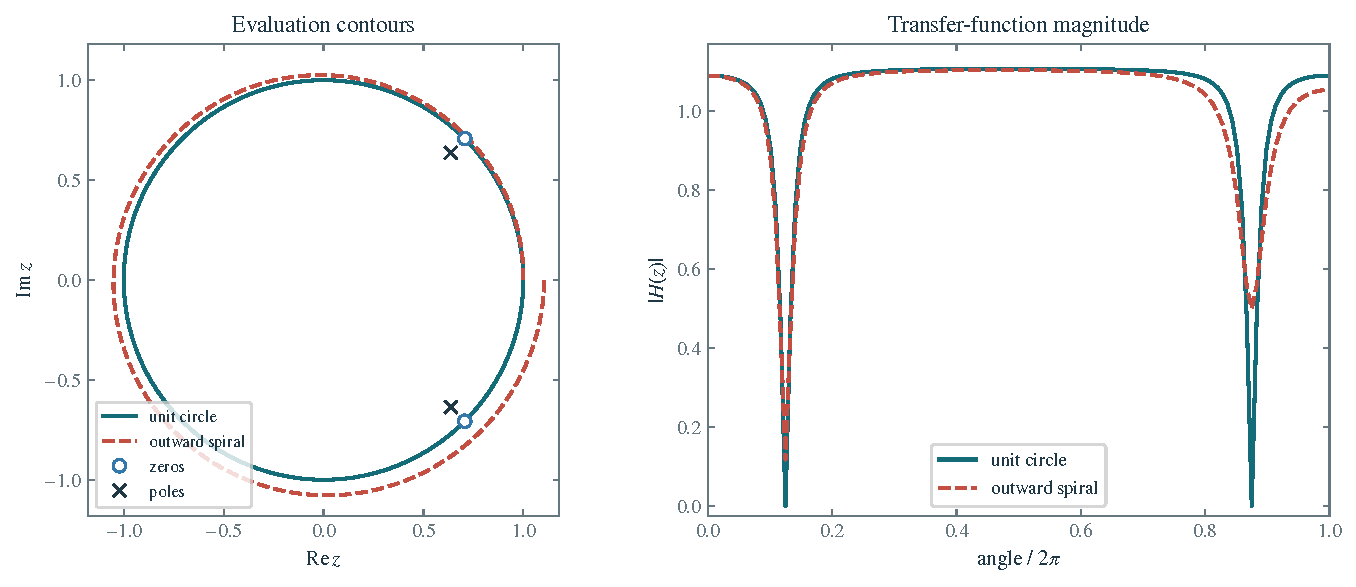
\includegraphics[width=\linewidth]{figures/chapter-related-transforms/z-transform-contours/figure.pdf}
\caption{The notch-filter transfer function evaluated on a unit circle and an outward logarithmic spiral. Both contours lie in the causal region of convergence; leaving the unit circle changes the depth of the notches.}
\label{fig-z-transform}
\end{figure}
Off the unit circle, the chirp factors can grow or decay rapidly. The
algebraic identity remains exact, but floating-point overflow and
cancellation can limit the accuracy of a direct chirp implementation.

\subsection{Computing a DFT of arbitrary length}
\label{sect2-applications-z-transform-tfd}
Choosing $z=e^{2\pi\imath/N}$ gives $\Gg_z=\Ff_N$. The chirp construction
therefore computes a DFT even when $N$ is prime. With $Q$ the smallest
power of two satisfying $Q\geq2N-1$, it needs two forward FFTs and one
inverse FFT of length $Q$, together with linear work. The kernel transform
can be cached for repeated inputs. Since $Q<4N$, the cost is
$O(N\log N)$, although its constant differs from a radix-two FFT.
This is Bluestein's algorithm; see~\cite{swarztrauber-bluestein}. Rader's alternative prime-length
construction is developed in Exercise~\ref{exo-chirp-transform-finis-corps}.
Appending zeros directly to the input also permits a longer FFT, but it
changes the frequency grid and does not by itself compute the original
length-$N$ DFT.

\section{Scaled-frequency Fourier transforms}
\label{sect1-transforme-fourier-fractionionnaire}
\subsection{Definition and computation}
\label{sect2-trans-frac}
For a real parameter $\alpha$, define
\[
 G(f,\alpha)[k]=\sum_{n=0}^{N-1}f[n]e^{-2\pi\imath\alpha nk/N},
 \qquad 0\leq k<N.
\]
This is $\Gg_z(f)$ with $z=e^{2\pi\imath\alpha/N}$ and can therefore be
computed by the CZT algorithm. It changes the spacing between sampled
frequencies. It is sometimes called a fractional Fourier transform~\cite{bailey-frac-trans},
but it is distinct from the unitary fractional powers of the normalized
DFT in Section~\ref{sect2-eigenvalues-tfd}.
For example,
\[
 G(f,1)=\Ff(f),\qquad G(f,-1)=N\Ff^{-1}(f),\qquad
 G(f,0)[k]=\sum_n f[n].
\]
The last map is not the identity for $N>1$. In general these transforms
are neither unitary nor a group under composition, and replacing $\alpha$
by $-\alpha$ does not give the inverse. Their usefulness here lies in
flexible spectral evaluation.
\begin{figure}[tbp]
\centering
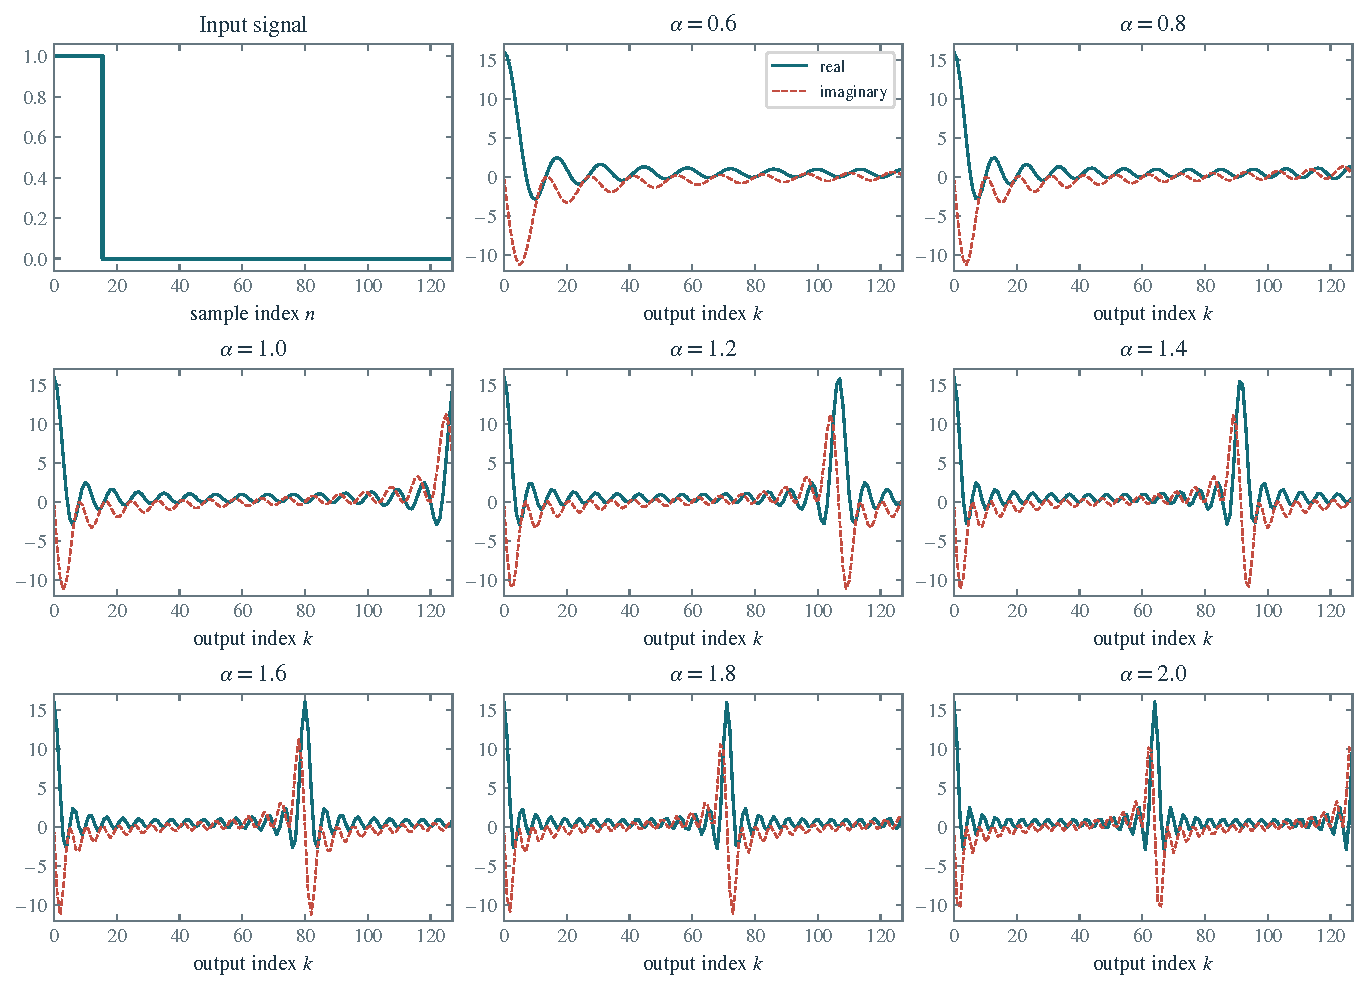
\includegraphics[width=\linewidth]{figures/chapter-related-transforms/scaled-fourier-signal/figure.pdf}
\caption{Scaled-frequency Fourier transforms of an interval indicator. The real and imaginary parts share the same scale. Changing $\alpha$ changes the sampled frequency grid.}
\label{fig-transforme-fourier-fractionionnaire-1d}
\end{figure}

\subsection{Finite records and spectral leakage}
\label{sect2-applications-trans-frac-periodicite}
\index{Spectral leakage}
A finite observation window spreads the spectrum of a sinusoid. Consider
$f[n]=e^{2\pi\imath\beta n/N}$ for $0\leq n<N$, and evaluate its
finite-record spectrum at any real frequency $\nu$:
\[
 S(\nu)=\sum_{n=0}^{N-1}e^{2\pi\imath(\beta-\nu)n/N},\qquad
 |S(\nu)|=\left|\frac{\sin\pi(\beta-\nu)}
                         {\sin(\pi(\beta-\nu)/N)}\right|.
\]
At removable singularities, where $\beta-\nu\in N\ZZ$, the magnitude is $N$.
If $\beta$ is an integer, the DFT grid samples the zeros of the sidelobes,
leaving a single nonzero bin. For noninteger $\beta$, the same windowed
spectrum is sampled away from those zeros. This is spectral leakage,
not a failure of the DFT to represent the finite vector.
\begin{figure}[tbp]
\centering
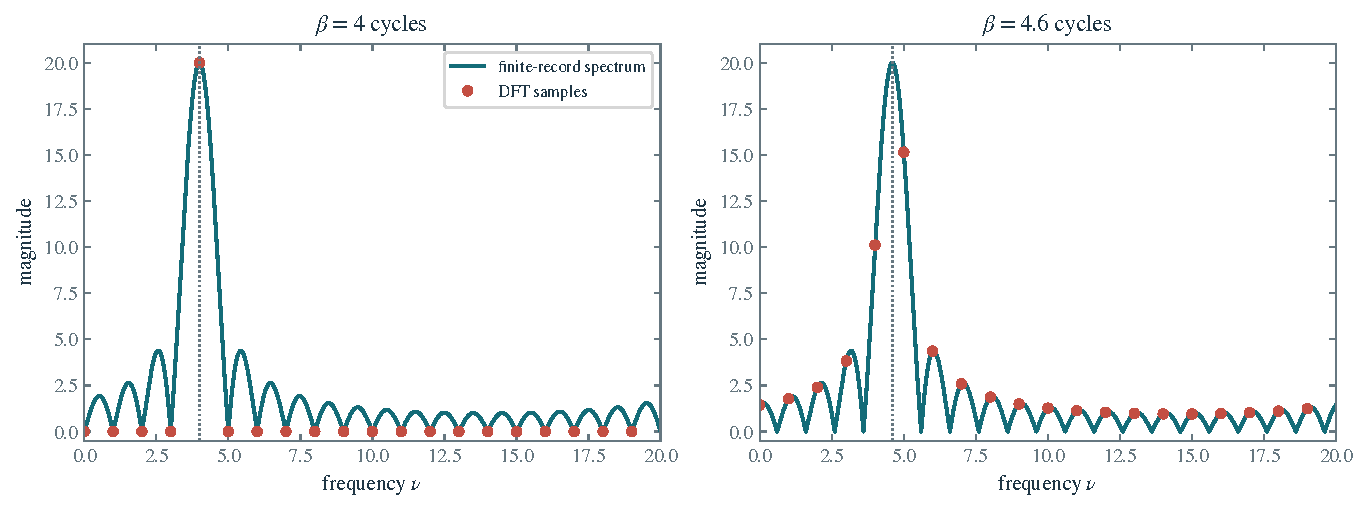
\includegraphics[width=\linewidth]{figures/chapter-related-transforms/spectral-leakage/figure.pdf}
\caption{Finite-record spectra of sinusoids with integer and noninteger numbers of cycles. The continuous curves evaluate the finite sum; the dots are DFT samples. The vertical line marks the generating frequency.}
\label{fig-spectrum-non-periodic-signal}
\end{figure}

\paragraph{Zooming around a spectral peak.}
To evaluate $S(b+k\delta)$ for $0\leq k<M$, modulate the data and use
an $M$-output chirp transform:
\[
 S(b+k\delta)=\sum_{n=0}^{N-1}
 \underbrace{f[n]e^{-2\pi\imath bn/N}}_{\widetilde f[n]}
 e^{-2\pi\imath\delta nk/N}.
\]
A coarse FFT can locate a neighborhood of a peak; the CZT then samples
that neighborhood densely without evaluating the entire frequency range.
For noisy or multitone signals, the peak location need not equal an
underlying component frequency exactly. Finer evaluation does not remove
noise, window effects, or sampling aliases.

\paragraph{Adjusting the observation length.}
For a pure tone with known $1<\beta<N/2$, set $b=\lfloor\beta\rfloor$,
$L=Nb/\beta$, and let $r$ be the nearest integer to $L$. Retain the first
$r\leq N$ samples and evaluate
\[
 F_k=\sum_{n=0}^{r-1}f[n]e^{-2\pi\imath kn/L}
     =G\bigl(f[0{:}r-1],r/L\bigr)[k],\qquad 0\leq k<r.
\]
Here $f[0{:}r-1]$ denotes the vector of those $r$ samples. This operation
\emph{shortens} the record. It is not zero padding, and changing frequency
spacing while retaining all $N$ samples would not have the same effect.
If $L=r$ is an integer, orthogonality gives $F_k=r\delta_b^k$.
Otherwise, write $s=r-L$, so $|s|\leq1/2$. Then $F_b=r$, and for $k\ne b$,
\[
 |F_k|=\left|\frac{\sin(\pi s(b-k)/L)}{\sin(\pi(b-k)/L)}\right|,
\]
with the usual limiting interpretation if the denominator vanishes.
For $0<|b-k|\leq L/2$, the elementary sine bounds imply
$|F_k|\leq\pi|s|/2\leq\pi/4$. Close to the peak, the ratio is approximately
$|s|$; farther away, small denominators can produce larger values.
This adjustment reduces leakage for the chosen tone, at the cost of
using fewer data and a frequency grid tailored to that tone.
\begin{figure}[tbp]
\centering
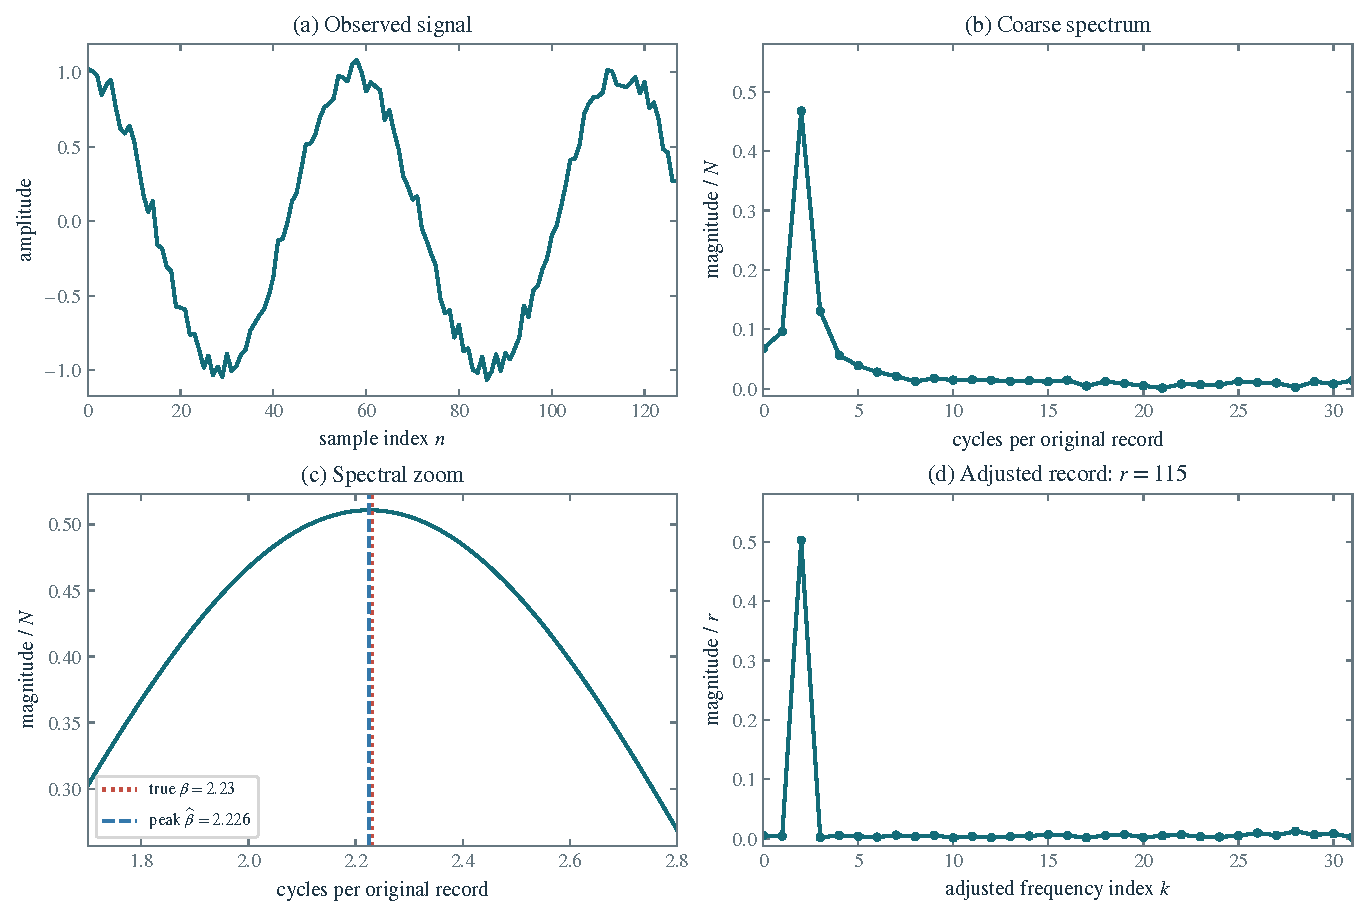
\includegraphics[width=\linewidth]{figures/chapter-related-transforms/spectral-zoom-and-adjustment/figure.pdf}
\caption{A noisy cosine, its coarse spectrum, a local spectral zoom, and an adjusted spectrum after shortening the record using the estimated peak. Spectral magnitudes are divided by the respective record lengths. The generating frequency is distinguished from its estimate.}
\label{fig-transforme-fourier-fractionionnaire}
\end{figure}

\section{Exercises}
\label{sect1-ext-trans-fourier-exercises}

\begin{exo}[Eigenvectors and powers of the Hartley transform]
\label{exo-eigenvectors-transfo-hartley}
Find the possible eigenvalues of $\Hh$ and construct the orthogonal
projectors onto the corresponding eigenspaces. Use these projectors to
define a continuous one-parameter group of unitary powers $V^t$ of
$V=\Hh/\sqrt N$, with $V^0=\Id$ and $V^1=V$. State the branch chosen
for the eigenvalue $-1$, and explain how to recover powers of the
unnormalized transform. Compare with the construction in
Section~\ref{sect2-eigenvalues-tfd}.
\begin{figure}[tbp]
\centering
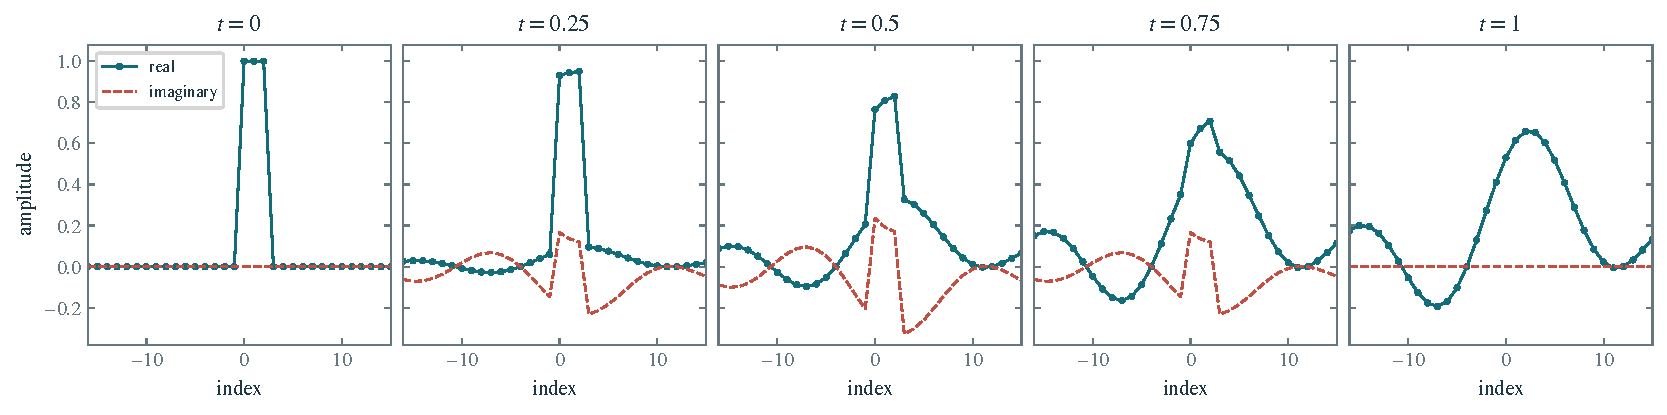
\includegraphics[width=\linewidth]{figures/chapter-related-transforms/fractional-hartley/figure.pdf}
\caption{Real and imaginary parts of fixed-branch unitary Hartley powers $V^t f$, with $V=\Hh/\sqrt N$. All panels use the same amplitude scale and preserve the norm.}
\label{fig-transfo-hartley-interm}
\end{figure}
\end{exo}

\begin{exo}[Generalized Hartley transform]
\label{exo-transfo-hartley-generalisee}
The identity
\begin{equation}
\label{eq-factorization-case}
 \cas x=\sqrt2\cos(x-\pi/4)
\end{equation}
suggests, for $N\geq3$, the family
\[
 \Hh_\lambda(f)[n]=\sum_{k=0}^{N-1}f[k]
                  \cos\left(\frac{2\pi nk}{N}+\lambda\right).
\]
Show that this map is invertible precisely when $\lambda$ is not an
integer multiple of $\pi/2$, and prove
\begin{equation}
\label{eq-inverse-hartley-generalized}
 \Hh_\lambda^{-1}=\frac{2}{N\sin(2\lambda)}\Hh_{\pi/2-\lambda}.
\end{equation}
Distinguish this family, which changes the kernel phase, from the
fractional powers in the preceding exercise.
\begin{figure}[tbp]
\centering
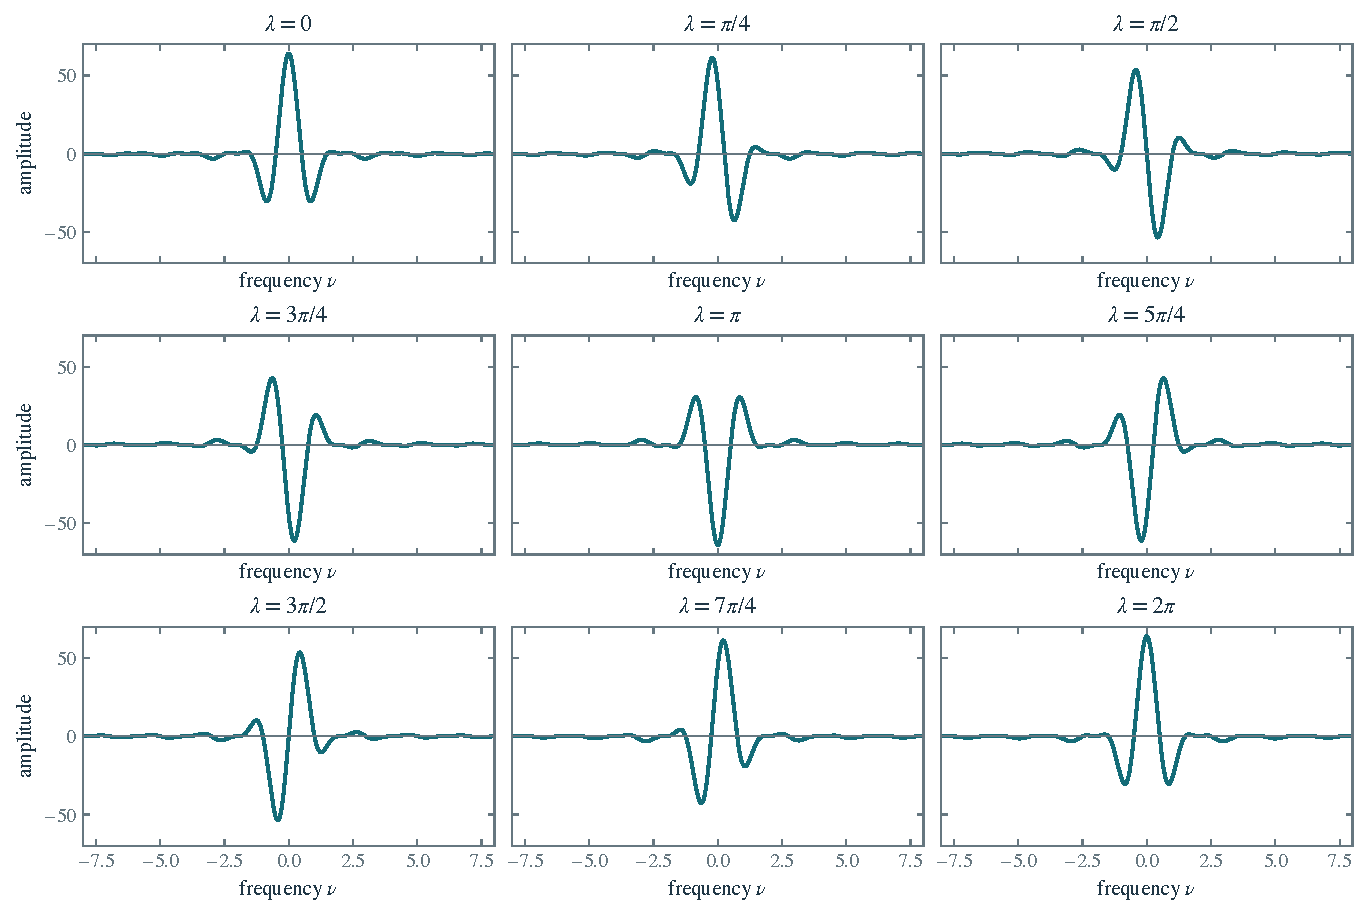
\includegraphics[width=\linewidth]{figures/chapter-related-transforms/generalized-hartley/figure.pdf}
\caption{Generalized Hartley transforms of the same triangular signal. The phase $\lambda$ changes the relative cosine and sine contributions; the two endpoint panels illustrate the $2\pi$ periodicity.}
\label{fig-transforme-hartley-generalized}
\end{figure}
\end{exo}

\begin{exo}[Interpolation by the Hartley transform]
\label{exo-interpolation-transfo-hartley}
Let $N=2K+1$ and $f\in\RR^N$. Construct the trigonometric polynomial with
frequencies $-K,\ldots,K$ that interpolates $f$ at the integers
$0,\ldots,N-1$, using its Hartley coefficients. Explain how centered
frequency padding evaluates it on a finer uniform grid. Prove that it is
the same interpolant as in Exercise~\ref{exo-interpolation-trigonometric},
and specify the normalization after padding.
\end{exo}

\begin{exo}[A separable two-dimensional Hartley transform]
\label{exo-transfo-hartley-2d}
For $f\in\RR^{N_1\times N_2}$ define
\[
 \Hh_2(f)[n_1,n_2]=\sum_{k_1=0}^{N_1-1}\sum_{k_2=0}^{N_2-1}
 f[k_1,k_2]\cas\frac{2\pi k_1n_1}{N_1}\cas\frac{2\pi k_2n_2}{N_2}.
\]
Prove $\Hh_2^2=N_1N_2\Id$ and give an algorithm based on row and column
transforms. This tensor-product convention uses a product of two
$\cas$ functions, not $\cas$ of the sum of the two phases.
\end{exo}

\begin{exo}[Hartley transforms over finite fields]
\label{exo-transfo-hartley-corps-finis}
Let $\FF_q$ have odd characteristic, let $\zeta$ have order $N$, and
suppose that the field contains $\iota$ with $\iota^2=-1$. Define a
Hartley kernel by replacing cosine and sine with
\[
 C_j=\frac{\zeta^j+\zeta^{-j}}2,\qquad
 S_j=\frac{\zeta^j-\zeta^{-j}}{2\iota}.
\]
Prove the inversion identity and derive a radix-two FHT when $N$ is a
power of two. Extend the argument to a commutative ring in which $2$ and
$N$ are units and $\zeta$ is a principal $N$th root of unity.
Implement an exact example in $\FF_5[X]/(X^4+3)$ with $N=16$ and $\iota=2$.
The finite-field constructions are developed in the next chapter.
\end{exo}

\begin{exo}[Chirp transforms and Toeplitz matrices]
\label{exo-chirp-transform-toeplitz}
Choose a logarithm $L$ of $z\ne0$ and set
$h[k]=f[k]e^{-Lk^2/2}$ and $g[j]=e^{Lj^2/2}$. Then
$y[n]=e^{Ln^2/2}\Gg_z(f)[n]=\sum_{k=0}^{N-1}g[n-k]h[k]$.
\begin{enumerate}
\item Show that $y=Th$ for a Toeplitz matrix $T$, and write $T$ when $N=3$.
\item A general $m\times n$ Toeplitz matrix has entries $T_{ij}=t_{i-j}$.
Denote its first column by $c=(t_0,\ldots,t_{m-1})$ and its first row by
$r=(t_0,t_{-1},\ldots,t_{-(n-1)})$. For $Q\geq m+n-1$, embed these data in
\[
 v=(c_0,\ldots,c_{m-1},\underbrace{0,\ldots,0}_{Q-m-n+1},r_{n-1},\ldots,r_1).
\]
Locate $T$ in the circulant matrix $C(v)$ with entries $v[i-j\bmod Q]$,
and use this embedding to compute $Tx$ by FFTs.
\item Apply the construction to the chirp kernel. Write the embedded
vector for $N=3$, $Q=8$, and implement the algorithm for $N$ input samples
and $M$ output values.
\end{enumerate}
\end{exo}

\begin{exo}[Quadrature methods as recursive filters]
\label{exo-meth-quadratures-recursive-filter}
For a continuous input, consider the integrator
$y(t)=\int_0^t x(\tau)\d\tau$. Find its zero-state Laplace transfer
function. Sample with spacing $\Delta>0$, and use the rules
\begin{equation}
\label{eq-defn-meth-quadrature}
\begin{aligned}
 (M_0)\quad\int_0^1 f(t)\d t&\approx f(0),\\
 (M_1)\quad\int_0^1 f(t)\d t&\approx\tfrac12(f(0)+f(1)),\\
 (M_2)\quad\int_0^1 f(t)\d t&\approx\tfrac16(f(0)+4f(1/2)+f(1)).
\end{aligned}
\end{equation}
Derive the left-rectangle and trapezoidal recurrences over one time step,
and Simpson's recurrence over two steps. Determine the corresponding
zero-state rational digital transfer functions. Explain the initialization
needed to approximate the integral from $0$, and identify the poles.
\end{exo}

\begin{exo}[Cubic spline prefiltering by recursions]
\label{exo-calcul-spline-iir}
Use the notation of Exercise~\ref{exo-spline-filtering} and the centered
cubic B-spline $\beta^3$.
\begin{enumerate}
\item Compute its integer samples $\beta_d^3$ and prove
$\Zz(\beta_d^3)(z)=(z+4+z^{-1})/6$.
\item Factor the reciprocal of this expression and write it as a sum of a
causal and an anticausal first-order transfer function, plus a constant.
Identify the common annulus of convergence that gives a stable inverse.
\item For data $u[0],\ldots,u[K-1]$ with $K\geq2$, impose whole-sample
mirror extension: $u[-j]=u[j]$ and $u[K-1+j]=u[K-1-j]$.
Derive exact endpoint initialization for the forward and backward
recursions, then compute the interpolation coefficients from their sum.
\item Derive an alternative cascade of the two filters, with exact mirror
initialization. Verify that both methods reproduce constant data and
satisfy the spline interpolation equations at every sample, including the
endpoints. See~\cite{unser-spline,unser-splines-perfect-fit} for the
filtering interpretation.
\end{enumerate}
\end{exo}

\begin{exo}[Rader's prime-length FFT]
\label{exo-chirp-transform-finis-corps}
Let $p$ be prime, $g$ a generator of $\FF_p^*$, and
$\omega_p=e^{2\pi\imath/p}$. For $f:\FF_p\to\CC$, show that
\[
 \wh f(g^{-b})=f(0)+\sum_{a=0}^{p-2}f(g^a)\omega_p^{-g^{a-b}},
 \qquad 0\leq b<p-1.
\]
Interpret this as a circular convolution on $\ZZ/(p-1)\ZZ$, specify its
inputs and the output permutation, and implement the algorithm. Keep the
zero-frequency coefficient separate.
\end{exo}

\begin{exo}[Fourier-integral quadrature on a flexible frequency grid]
\label{exo-calcul-approaches-transfo-frac}
Let $f$ be continuous on $[a_0,a_0+a]$ and zero outside. The desired
frequencies are $\xi_k=\xi_0+k\delta$ for $0\leq k<M$.
\begin{enumerate}
\item Use the left-rectangle samples $x_j=a_0+jh$, $0\leq j<N$,
with $h=a/N$, to approximate
$\wh f(\xi_k)=\int f(t)e^{-\imath\xi_kt}\d t$ by one chirp transform.
Specify the modulation, chirp parameter, outer phase, and factor $h$.
If $h\delta/(2\pi)=p/q$ in lowest terms, explain how the same finite sum
can be read from a suitably padded DFT of length a multiple of $q$.
Compare this with the chirp construction when $q$ is large.
\item Replace the rule by composite Simpson quadrature on an odd number
$N\geq3$ of samples \emph{including both endpoints}, now with
$h=a/(N-1)$. Give the weights and implement the approximation with all
physical scaling and phase factors included.
\end{enumerate}
\end{exo}

\begin{exo}[Scaled-frequency transforms of an image]
\label{exo-transforme-fourier-fractionionnaire-2d}
Extend $G(f,\alpha)$ to rectangular two-dimensional arrays by tensor
product. Write a Python function that applies the transform along both
axes, and check that $\alpha=1$ gives the usual two-dimensional DFT.
Test it on a disk indicator, displaying the magnitude of the complex output.
\begin{figure}[tbp]
\centering
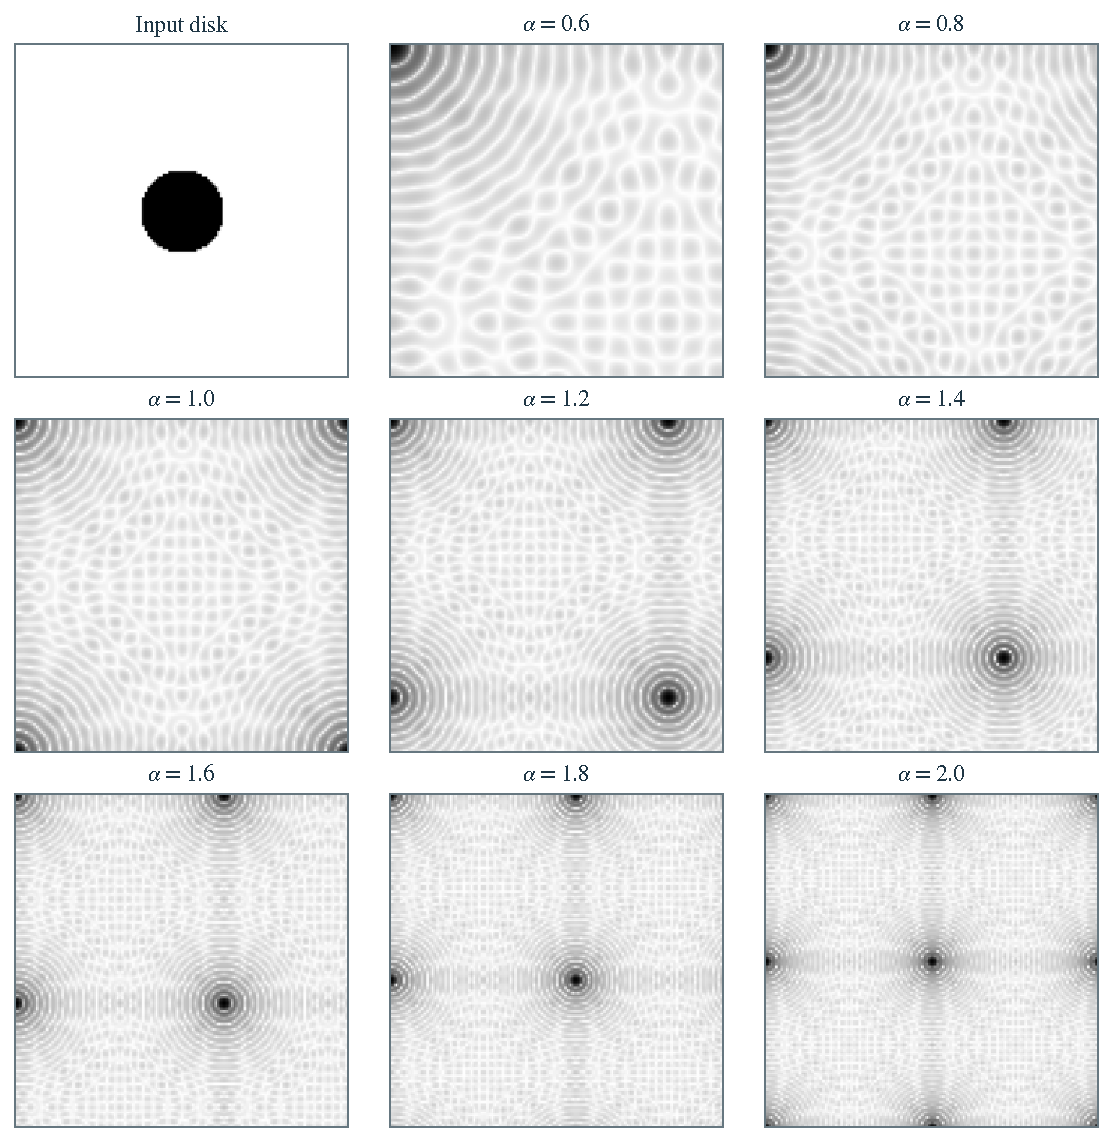
\includegraphics[width=.82\linewidth]{figures/chapter-related-transforms/scaled-fourier-image/figure.pdf}
\caption{Magnitudes of scaled-frequency two-dimensional Fourier transforms of a disk. Spectral panels share the contrast mapping $\log(1+100|G_2|/\sum f)/\log(101)$, shown dark on white; the input panel uses ordinary grayscale.}
\label{fig-transforme-fourier-fractionionnaire-2d}
\end{figure}
\end{exo}
